\section{Methodology}
It is easy to notice that that the nested $i$ and $j$ for-loops in Alg. \ref*{alg:fw1} are totally independent and therefore parallelizable. \\
In this section we describe three strategies to overcome the iniefficiency due to a mono-thread computation.


\subsection{Distributed with MPI}

....



\begin{lstlisting}[style=CStyle]
...
int processes, rank;

MPI_Init(&argc, &argv);

MPI_Comm_size(MPI_COMM_WORLD, &processes);
MPI_Comm_rank(MPI_COMM_WORLD, &rank);

MPI_Bcast(&n, 1, MPI_INT, 0, MPI_COMM_WORLD);

populateMatrix(matrix, n, density, rank, processes);

int k, i, j, temp;
int* kRow = malloc(n*sizeof(int));
int section = n / processes;

for (k = 0; k < n; k++) 
{
	
	castKRow(matrix, n, section, kRow, k, rank);
	
	for (i = 0; i < section; i++)
	{
		for (j = 0; j < n; j++) 
		{
			temp = matrix[i * n + k] + kRow[j];
			if (temp < matrix[i * n + j])
			{
				matrix[i * n + j] = temp;
			}
		}
	}
}

gatherResult(matrix, n, rank, processes);
\end{lstlisting}





































































\subsection{Multithreading with OpenMP}
OpenMP (Open Multi-Processing) is an application programming
interface (API) for parallel programming intended to work on shared-
memory architectures. More specifically, it is a set of compiler
directives, library routines and environmental variables, which in-
fluence run-time behavior. OpenMP enables parallel programming in
various languages, such as C, C++ and FORTRAN and runs on most
operating systems. \par
The OpenMP API uses the fork-join model of parallel execution.
Multiple threads perform tasks defined implicitly or explicitly by
OpenMP directives. All OpenMP applications begin as a single thread
of execution, called the initial thread. The initial thread executes
sequentially until it encounters a parallel construct. At that point,
this thread creates a group of itself and zero or more additional
threads and becomes the master thread of the new group. Each thread
executes the commands included in the parallel region, and their
execution may be differentiated, according to additional directives
provided by the programmer. At the end of the parallel region, all
threads are synchronized. \par
The runtime environment is responsible for effectively scheduling
threads. Each thread, receives a unique id, which differentiates it
during execution. Scheduling is performed according to memory
usage, machine load and other factors and may be adjusted by altering
environmental variables. In terms of memory usage, most variables in
OpenMP code are visible to all threads by default. However, OpenMP
provides a variety of options for data management, such as a thread-
private memory and private variables, as well as multiple ways of
passing values between sequential and parallel regions. Additionally,
recent OpenMP implementations introduced the concept of tasks,
as a solution for parallelizing applications that produce dynamic
workloads. Thus, OpenMP is enriched with a flexible model for
irregular parallelism, providing parallel while loops and recursive
data structures. \par
The main advantage on using OpenMP is the ease of developing parallelisms
with simple constructs that do not differ too much from the original implementation.

The following snippet shows the implementation used in this work: the matrix containing the
distances between vertices is shared among all the threads, while the 3 nested for-loops are executed
by each thread indipendentely.



\begin{lstlisting}[style=CStyle]
int i, j, k;
#pragma omp parallel num_threads(t) shared(M) private(k) {
	for(k = 0; k < n; k++) {
		#pragma omp for private(i,j) schedule(dynamic)			
		for(i = 0; i < n; i++) {
			for(j = 0; j < n; j++) {
				if(M[i][j] > M[i][k] + M[k][j] || M[i][j] == 0) {
					M[i][j] = M[i][k] + M[k][j];
				}
			}
		}
	}
}
\end{lstlisting}

A dynamic scheduler works better than a static one in this case because the
density of the edges may vary and the compiler cannot foresee the content of the matrix. \\
Also note that the solution does not implement a \texttt{collapse} directive like this:
\begin{lstlisting}[style=CStyle]
...
#pragma omp for ... collapse(3)
for(k = 0; k < n; k++) {			
	for(i = 0; i < n; i++) {
		for(j = 0; j < n; j++) {
			...
		}
	}
}
\end{lstlisting}
that's because when we collapse a multiple loops, OpenMP turns the into a single loop: there is a single
index that is constructed from \texttt{i}, \texttt{i} and \texttt{k} using division and modulo operations. This can
have huge impact on the performance because of the overhead, especially if the matrix is really wide.

\textbf{Figure \ref*{fig:threads}} shows how 2 threads interact inside the matrix: the red and orange zones highlight the cells where
Thread 1 and Thread 2 can write respectively; the blue and turquise cells represent the intermediate vertices that are compared
with the vertice under analysis for Thread 1 and Thread 2 respectively.

\begin{figure}[h!]
\centering                                                                        
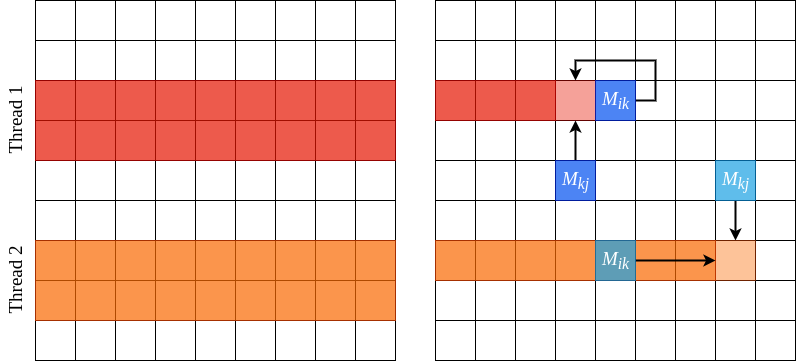
\includegraphics[width=3.5in]{diagrams/openmp-threads}
\captionsetup{justification=centering,margin=2cm}                                                                                                                                   
\caption{View of the data each thread can reach}                                                                                                                                            
\label{fig:threads}                                                                                                                                                           
\end{figure}

It may seems that this implementation is affected by data races, because there's no lock when writing in \texttt{M} 
and one of the intermediate cells could be the same under analysis on another thread; for example, Thread 1 could write
in cell $M_{i,j}$ before or after that Thread 2 calculates $M_{x,j} > M_{x,i} + M_{i,j}$, making the result unpredictable.

We prove that no race condition may appear in this case. Let's assume we have 2 threads, namely $T^1$ and $T^2$ and they are
analyzing cell $(i,j)$ and $(x,y)$, with $x \neq i$. We denote the previous statement simply with $T^{1}_{i,j}$ and $T^{2}_{x,y}$.
Having in common $k$, the two threads are now calculating the following system

\begin{flalign}\label{eq:sys1}
 &&  \left\{\begin{matrix}
T^{1}_{i,j} & > & T^{1}_{i,k} & + & T^{1}_{k,j} \\
\\ 
T^{2}_{x,y} & > & T^{2}_{x,k} & + & T^{2}_{k,y}
\end{matrix}\right. &&
\end{flalign}

The two inequalities are taken from the condition of the \emph{if} condition in \textbf{Algorithm \ref*{alg:fw1}}. \\ 
If both are true, then $T^{1}$ and $T^{2}$ are allowed to write in $M$. In order to have a data race condition, the following
must be true
\[(k = i \wedge y = j) \vee (x = i \wedge k=j)\]
but since $x \neq i$, only the following must be verified

\begin{flalign}\label{eq:cond1}
 &&  k = i \wedge y = j &&
\end{flalign}
By applying (\ref*{eq:cond1}) to (\ref*{eq:sys1}) we have

\begin{flalign}\label{eq:sys2}
 &&  T^{1}_{i,j} > T^{1}_{k,k} + T^{1}_{i,j} &&
\end{flalign}
but (\ref*{eq:sys2}) is clearly false, because $M$ is a hollow matrix \emph{i.e.} the  diagonal elements are all equal to $0$, leaving the 
following inequality:
\begin{flalign}\label{eq:sys3}
 &&  T^{1}_{i,j} > T^{1}_{i,j} &&
\end{flalign}
Clearly no number can be greater than itself and this means that only $T^2$ may write in $M$ at this point. \\
No race condition can appear if $k$ is the same among the threads and threrfore there's no need to verify atomicity of the write operation;
the lack of OpenMP directive like \texttt{atomic} or \texttt{critical} plays in favor of performance. \par

The speedup of the solution is sligthy worse than the ideal speedup (see \textbf{Figure \ref*{fig:omp-speedup}})

\begin{figure}[h!]
\centering                                                                        
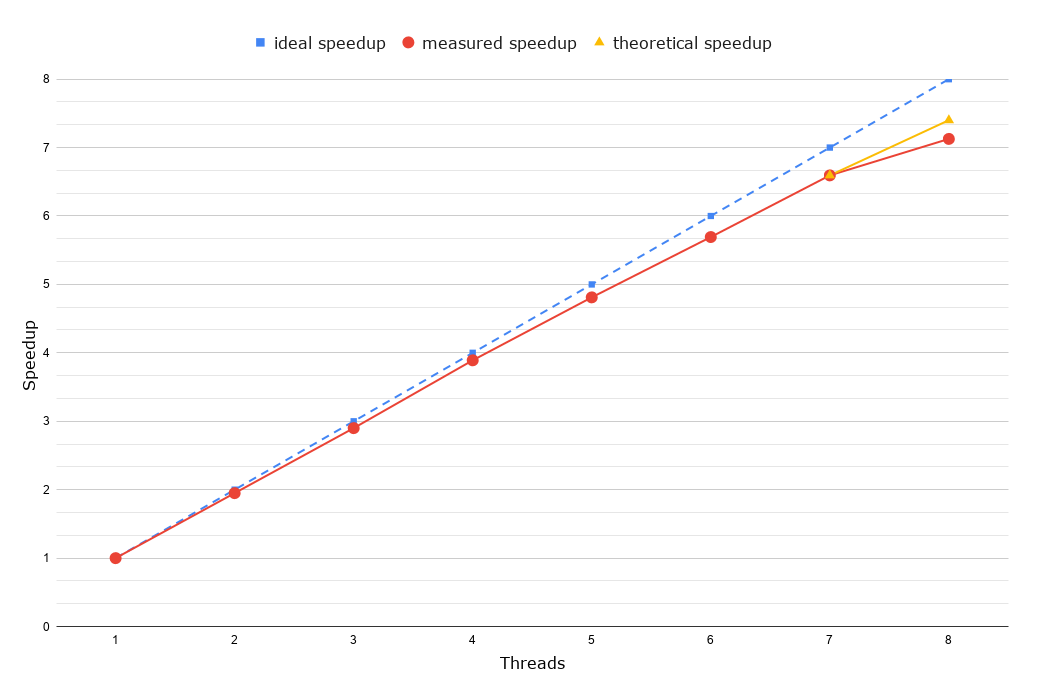
\includegraphics[width=3.5in]{diagrams/openmp-speedup}
\captionsetup{justification=centering,margin=2cm}                                                                                                                                   
\caption{Speedup of \emph{OpenMP} FW on a octacore CPU}                                                                                                                                            
\label{fig:omp-speedup}                                                                                                                                                           
\end{figure}
When scaling from 7 to 8 threads, we notice a slight deviation from the previous (almost) linear trend. That's because the measurement
is taken from a 8-core/8-thread CPU, namely Intel Core i7-9700K, and because no other cores were free to manage the OS and its subprocesses, the scheduler
divided this task among all the threads. So we have approximated the speedup without counting the fluctuations due to the management of the OS. \par

The efficiency, which stays always above $90\%$, is shown in \textbf{Figure \ref*{fig:omp-efficiency}} alongside with its theoretical counterpart.

\begin{figure}[h!]
\centering                                                                        
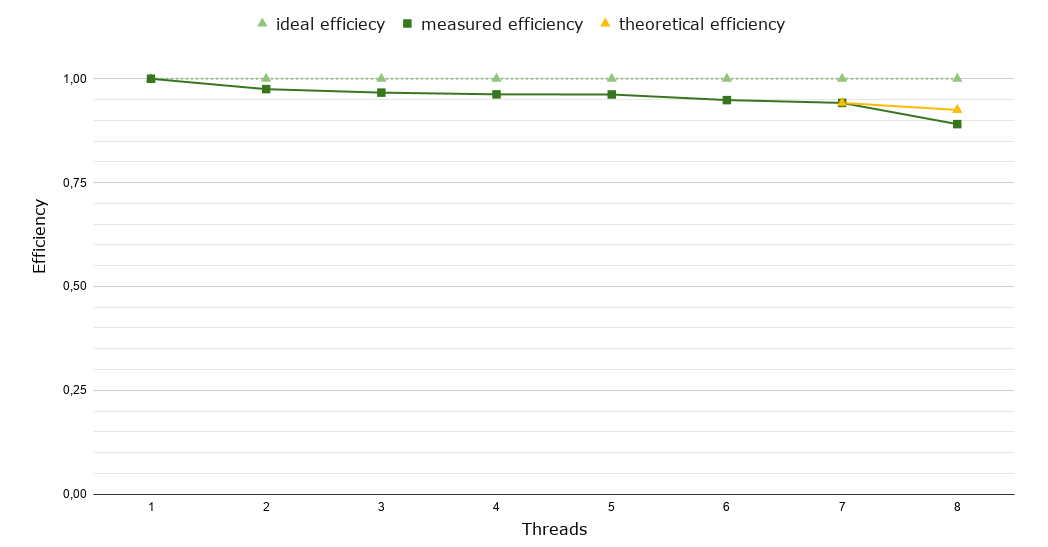
\includegraphics[width=3.5in]{diagrams/openmp-efficiency}
\captionsetup{justification=centering,margin=2cm}                                                                                                                                   
\caption{Efficiency of \emph{OpenMP} FW on a octacore CPU}                                                                                                                                            
\label{fig:omp-efficiency}                                                                                                                                                           
\end{figure}
An overview of the timings collected can be found in \textbf{Table \ref*{tab:omp-time}}.













































































\subsection{GPGPU with CUDA}